% AI4SE Workshop @ KI 2026 — Expanded Literature Review Draft
% Springer LNCS format — EXPANDED beyond 4 pages, to be condensed later
\documentclass[runningheads]{llncs}

\usepackage[T1]{fontenc}
\usepackage{graphicx}
\usepackage{hyperref}
\usepackage{microtype}
\usepackage{booktabs}
\usepackage{xcolor}
\usepackage{tikz}
\usepackage{pgfplots}
\pgfplotsset{compat=1.18}

\begin{document}

\title{Memory-Aware Software Engineering Agents:\\ Architectures, Mechanisms, and Open Gaps}

\titlerunning{Memory-Aware SE Agents}

\author{Michael Banf, Johannes Kuhn, Slawomir Garcarz \and Max Becker}

\authorrunning{Banf et al.}

\institute{Perelyn GmbH, Munich, Germany\\
\email{michael.banf@perelyn.com}}

\maketitle

\begin{abstract}
AI-assisted software engineering has progressed from code completion to
agentic systems operating across the full development lifecycle. Yet
these agents remain fundamentally stateless: each task begins without
memory of prior sessions, resolved bugs, or accumulated project
understanding. We present a systematic review that synthesizes
evidence from a feature-level
analysis of ten production software engineering harnesses as well as a quantitative
classification the current state of the art memory architecture
for software engineering agents research. 

Our analysis reveals an episodic-temporal deficit, i.e.
59\% of workshop papers address episodic memory, yet only 4\% implement
temporal mechanisms beyond timestamps. 
That's the core paradox — researchers work on it, tools don't ship it

The LoCoMo-Plus experiment
confirms a structural 35--45 percentage-point factual-to-cognitive gap
across all three major memory paradigms. To this end, we identify several open gaps, from cross-session experiential learning and temporal consistency of
architectural knowledge to collaborative team memory and memory
governance. We argue that
persistent, structured, temporally grounded memory is the architectural
prerequisite for software agents that learn alongside the teams they serve.

\keywords{Software Engineering Agents \and Agentic Memory \and
Context Engineering \and Temporal Reasoning \and Knowledge Graphs}
\end{abstract}

%%% ==================================================================
\section{Introduction}\label{sec:intro}
%%% ==================================================================

Agentic AI systems now operate across the full software engineering
lifecycle~\cite{becker2026,liu2024survey,jimenez2024swebench}. Whether
resolving complex bugs through multi-file analysis, discovering
architectural patterns, or coordinating code reviews across a team, these
agents accumulate significant task-specific knowledge during each
session. Yet that knowledge vanishes when the session ends: the next
invocation begins from scratch, repeating investigations, rediscovering
constraints, and re-learning project conventions.

The field has responded rapidly to the memory challenge in general:
from approximately 25 papers in 2023 to over 200 in
2025~\cite{hu2025survey}, with every major AI provider now shipping
persistent memory alongside a maturing open-source ecosystem.
The ICLR\,2026 MemAgents workshop accepted 70 papers from 110+
submissions~\cite{memagents2026}, signaling that memory has become a
first-class research topic. Yet our classification reveals that
software engineering is dramatically under-represented with only 4 of
70 workshop papers (5.7\%) targeting software engineering tasks, and none addressing temporal
versioning, team-shared memory, or decision provenance.

%%% ==================================================================
\section{Memory in Production Software Engineering Harnesses}\label{sec:harnesses}
%%% ==================================================================

The CoALA taxonomy~\cite{sumers2024} maps human memory types onto agent
components: \emph{working} (context window), \emph{semantic}
(conventions, facts), \emph{episodic} (past debugging experiences),
\emph{procedural} (workflows, tool usage). Applied to software
engineering~\cite{banf2026}: working memory is well-served by modern
context windows; semantic memory is partially addressed by context
files~\cite{agentreadmes2025}; episodic and procedural memory are almost
entirely absent. A finer-grained functional taxonomy~\cite{hu2025survey}
distinguishes \emph{factual} (what the agent knows), \emph{experiential}
(what the agent has learned from doing), and \emph{working} memory
(active context management) with all three being critical for software engineering agents
operating over long project horizons. 

From this perspective, we analyzed the memory mechanisms of ten widely-used SE agent
harnesses as of mid-2026. Table~\ref{tab:harness} summarizes the
comparison across six key dimensions derived from the CoALA taxonomy.

\begin{figure}[h!]
\centering
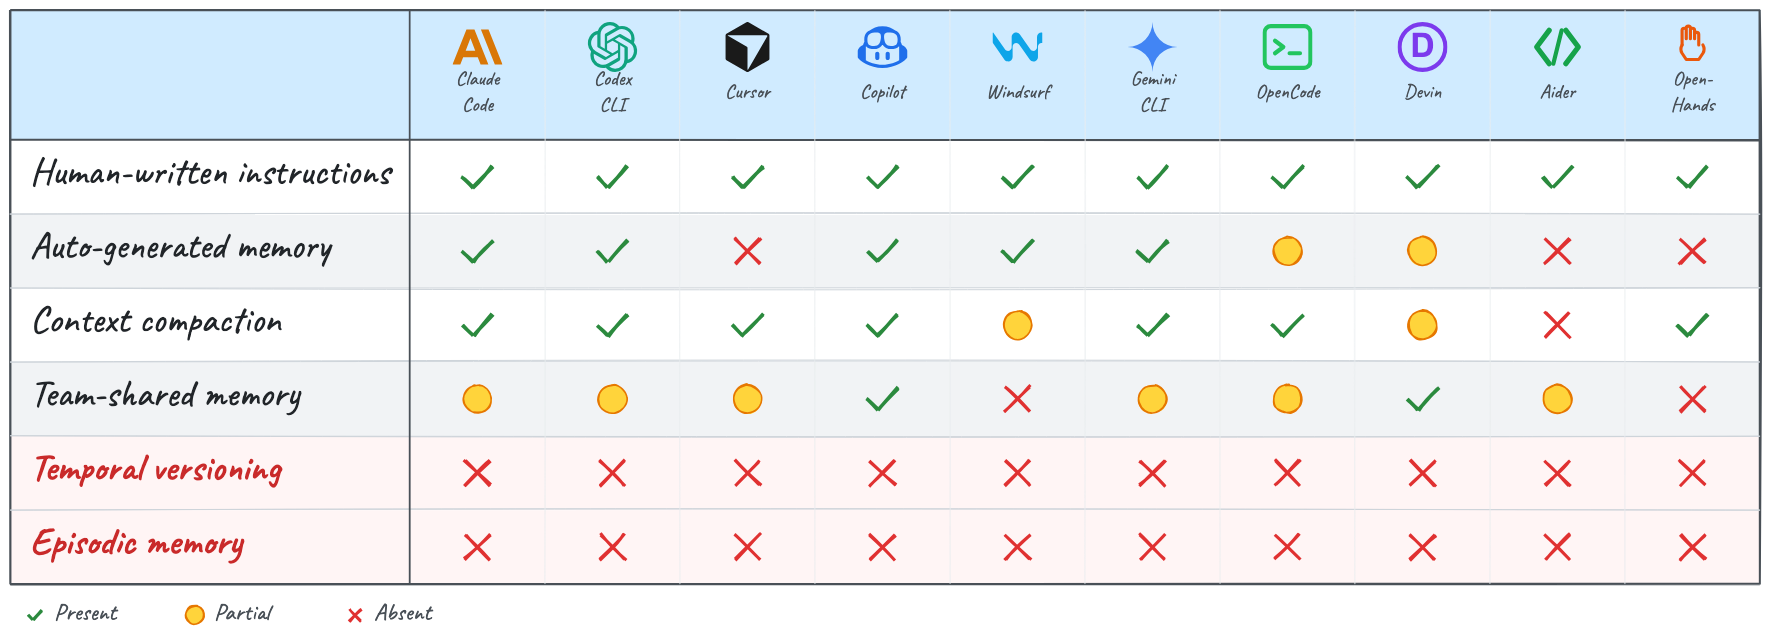
\includegraphics[width=\textwidth]{figures/harness-table.png}
\caption{Memory mechanisms in production software engineering harnesses.}
\label{tab:harness}
\end{figure}

% \begin{table}[h!]
% \caption{Memory mechanisms in production software engineering harnesses. \\
% $\bullet$\,=\,present, $\circ$\,=\,absent, $\triangle$\,=\,partial.}
% \label{tab:harness}
% \centering\footnotesize
% \setlength{\tabcolsep}{2.5pt}
% \begin{tabular}{@{}lcccccccccc@{}}
% \toprule
%  & \rotatebox{75}{Claude Code}
%  & \rotatebox{75}{Codex CLI}
%  & \rotatebox{75}{Cursor}
%  & \rotatebox{75}{Copilot}
%  & \rotatebox{75}{Windsurf}
%  & \rotatebox{75}{Gemini CLI}
%  & \rotatebox{75}{OpenCode}
%  & \rotatebox{75}{Devin}
%  & \rotatebox{75}{Aider}
%  & \rotatebox{75}{OpenHands} \\
% \midrule
% Human-written instructions & $\bullet$ & $\bullet$ & $\bullet$ & $\bullet$ & $\bullet$ & $\bullet$ & $\bullet$ & $\bullet$ & $\bullet$ & $\bullet$ \\
% Auto-generated memory      & $\bullet$ & $\bullet$ & $\circ$   & $\bullet$ & $\bullet$ & $\bullet$ & $\triangle$ & $\triangle$ & $\circ$ & $\circ$ \\
% Context compaction          & $\bullet$ & $\bullet$ & $\bullet$ & $\bullet$ & $\triangle$ & $\bullet$ & $\bullet$ & $\triangle$ & $\circ$ & $\bullet$ \\
% Team-shared memory          & $\triangle$ & $\triangle$ & $\triangle$ & $\bullet$ & $\circ$ & $\triangle$ & $\triangle$ & $\bullet$ & $\triangle$ & $\circ$ \\
% Temporal versioning         & $\circ$ & $\circ$ & $\circ$ & $\circ$ & $\circ$ & $\circ$ & $\circ$ & $\circ$ & $\circ$ & $\circ$ \\
% Episodic memory             & $\circ$ & $\circ$ & $\circ$ & $\circ$ & $\circ$ & $\circ$ & $\circ$ & $\circ$ & $\circ$ & $\circ$ \\
% \bottomrule
% \end{tabular}
% \end{table}

All ten harnesses support human-written instruction files (CLAUDE.md,
AGENTS.md, .cursorrules, copilot-instructions.md, GEMINI.md). This
represents the \emph{declarative semantic memory} layer, i.e. manually
authored project conventions injected into every prompt. Adoption is
widespread: Chatlatanagulchai et al.~\cite{agentreadmes2025} find over
60K repositories containing agent context files. Yet rigorous
evaluation~\cite{gloaguen2026} reveals developer-written files improve
issue resolution by only $\sim$4\% while increasing cost by 20\%;
LLM-generated files provide no measurable benefit on SWE-Bench. Context
engineering~\cite{contexteng2026} formalizes the approach, but all
implementations remain manually authored without temporal metadata.

Five harnesses now generate memories automatically, including Claude Code, Codex
CLI, Copilot, Windsurf, Gemini CLI, but approaches vary substantially:
Claude Code uses a two-phase extraction with user approval; Codex CLI
performs post-session memory extraction; Gemini CLI scans idle sessions.
Three tools (Cursor, Aider, OpenHands) have no auto-memory at all.
Critically, none distinguishes between factual knowledge (``this project
uses PostgreSQL 15'') and experiential knowledge (``the auth module
requires careful transaction handling because of race condition X'').

Context compaction triggers range from 75\% window utilization
in OpenCode to 95\% as in Cursor. All implementations are lossy:
technical details, intermediate reasoning steps, and
failed-approach information are discarded. SWE Context
Bench~\cite{zhu2026} demonstrates this problem quantitatively:
summarized experience improves resolution by +8.1~pp, while unfiltered
context hurts by $-$4.0~pp. The quality of compaction determines
whether memory helps or hinders.

No production software engineering agent supports temporal versioning, i.e. tracking when
knowledge was valid, when it changed, when it became stale. Neither do they support
episodic memory, i.e. structured records of past debugging sessions,
resolution trajectories, or decision rationale. This is the central
finding: the memory capabilities most critical for software engineering agents that
learn over time are precisely those that no tool implements.


%%% ==================================================================
\section{Memory Architectures: From Extraction to Graphs}\label{sec:architectures}
%%% ==================================================================

Three production paradigms have emerged for persistent agent
memory~\cite{hu2025survey,gurawaliya2026}, including extraction-based,
self-managing, and graph-based temporal, each with different strengths and weaknesses.

%%% ------------------------------------------------------------------
\subsection{Extraction-Based Memory}
%%% ------------------------------------------------------------------

Extraction-based architectures, such as Mem0~\cite{mem0_2025}, extracte atomic facts from conversations and store
them as vector-indexed entries. The pipeline consists of: i)~LLM-based
extraction of discrete facts, ii)~embedding and vector storage, and 
iii)~similarity-based retrieval at query time.

\paragraph{Strengths:} Extraction-based systems excel at
\emph{factual recall}: Mem0 achieves 63.0\% on the LoCoMo-Plus factual
benchmark~\cite{gurawaliya2026}, the highest among the three paradigms.
For software engineering tasks requiring explicit knowledge retrieval (``what database does
this project use?'', ``what are the coding conventions?''), this paradigm
is well-suited. It is also the simplest to integrate: Mem0's graph-enhanced
variant (Mem0g) adds entity-relation extraction atop the vector store.
For comparison, Zep achieves 94.8\% on the Deep Memory Retrieval
benchmark using its temporal knowledge graph~\cite{rasmussen2025}.

\paragraph{Limitations:} Extraction is lossy by design: the
process of converting rich debugging sessions into atomic facts discards
causal chains, temporal context, and reasoning paths. The LoCoMo-Plus
cognitive benchmark reveals this sharply: Mem0 drops from 63.0\% factual
to 18.0\% cognitive, i.e. a 45.0~pp gap~\cite{gurawaliya2026}.
Mem0's weakest category is \emph{state} at 15.0\%, precisely the kind of
context software engineering agents need: tracking evolving project state, developer
intent, and work-in-progress. On the retrieval-vs-utilization diagnostic
of \cite{diagnosing2026}, retrieval method dominates write strategy:
accuracy spans 20~pp across retrieval methods but only 3--8~pp across
write strategies, suggesting that raw chunked storage (zero LLM calls)
matches or outperforms expensive extraction.

%%% ------------------------------------------------------------------
\subsection{Self-Managing Memory}
%%% ------------------------------------------------------------------

Self-Managing Memory, such as Letta~\cite{packer2023}, treats the LLM itself as an operating system
managing its own memory via explicit read/write/search operations over a
hierarchical store. The agent decides what to remember and how to
organize it.

\paragraph{Strengths:} Self-managing memory excels at preserving
\emph{behavioral continuity}: goals, recurring patterns, and evolving
state. Letta leads the LoCoMo-Plus cognitive benchmark at 24.2\%
overall, with the highest single-category score on \emph{goal reasoning}
(30.0\%) and \emph{state reasoning} (28.0\%)~\cite{gurawaliya2026}.
For software engineering agents that must maintain an evolving picture of project
architecture, track long-running refactoring goals, or remember
what patterns emerged during debugging, self-managing memory is the
strongest fit.

\paragraph{Limitations:} Self-managing memory is less transparent
than explicit stores: the agent's internal state cannot easily be
inspected, audited, or corrected by developers. The Letta--Mem0 gap is
statistically significant after Holm correction ($p = 0.040$), but
Letta still achieves only 24.2\% on cognitive tasks, which is well below
what teams would need for reliable cross-session learning.

%%% ------------------------------------------------------------------
\subsection{Graph-Based Temporal Memory}
%%% ------------------------------------------------------------------

Graph-Based temporal approaches, such as Graphiti~\cite{rasmussen2025}, can distinguish \emph{event time} (when
something happened) from \emph{ingestion time} (when the system learned
it), with every edge carrying explicit validity intervals. This
\emph{bi-temporal} approach is unique among production memory systems.

\paragraph{Strengths:} Graph-based memory excels at \emph{causal
reasoning}: Zep leads decisively on causal tasks at 20.8\%, well ahead
of Mem0's 11.9\% and Letta's 12.9\%~\cite{gurawaliya2026}. It is also
the most consistent performer across all four cognitive dimensions (range:
20.8--25.0\%). For software engineering tasks requiring understanding of \emph{why} a
decision was made, how events connect across time, or what caused a
regression, temporal graphs provide the most natural representation.
On LongMemEval, Zep achieves 71.2\% using only 1.6K context tokens
versus 115K for full-context baselines~\cite{rasmussen2025} which is critical
for token-constrained SE agents.

\paragraph{Limitations:} Graph construction adds latency and
complexity. Zep does not lead on aggregate cognitive score (22.2\% vs.\
Letta's 24.2\%), and its advantage on causal reasoning may not offset
weaker goal/state tracking for many use cases. No software engineering specific
temporal graph system exists yet.

%%% ------------------------------------------------------------------
\subsection{Hybrid and Emerging Approaches}
%%% ------------------------------------------------------------------

The LoCoMo-Plus results make a compelling case for \emph{hybrid
architectures}, since no single paradigm masters all competency
types~\cite{gurawaliya2026}, 59.1\% were
answered incorrectly by all three systems and only 6.7\%
are correctly answered by all. The analysis confirms that
the systems capture genuinely different aspects of the memory problem. To this end several emerging directions point toward future software engineering relevant
architectures.

Reinforcement learning based memory management, such as Memory-R1~\cite{memoryr1_2025} and AgeMem~\cite{agemem2026} replace
heuristic memory policies with trained ones for ADD/ UPDATE/ DELETE
operations. The learned policies discover non-obvious strategies such as
preemptive summarization before the context window fills. Both remain
early-stage but suggest a path toward adaptive memory management tuned
to software engineering specific reward signals such as issue resolution rate, code quality
metrics.

Multi-graph memory, as in MAGMA~\cite{magma2026}, represents each memory item across orthogonal
semantic, temporal, causal, and \emph{entity} graphs, with retrieval
formulated as policy-guided traversal. This decomposition offers
fine-grained control particularly relevant for software engineering: dependency
relationships (entity graph), decision provenance (causal graph),
API validity (temporal graph), and conceptual similarity (semantic
graph) can be queried independently.

Hierarchical consolidation provides a formal theory of hierarchical memory~\cite{hierarchicalmemory2026}
defines three operators, i.e. extraction ($\alpha$), coarsening
($C = (\pi, \rho)$), and traversal ($\tau$). This identifies a
\emph{self-sufficiency spectrum} for representative functions that
constrains viable retrieval strategies. TiMem~\cite{timem2026}
implements this via a Temporal Memory Tree, reaching 75.3\% on LoCoMo
while reducing recalled tokens by 52\%. For software engineering agents processing
long execution traces, hierarchical consolidation is essential.


%%% ==================================================================
\section{Memory Mechanisms for Software Engineering}\label{sec:semechanisms}
%%% ==================================================================

Beyond general-purpose memory architectures, several mechanisms have
been developed specifically for or with direct relevance to software engineering agents.

%%% ------------------------------------------------------------------
\subsection{Versioned Context Management}
%%% ------------------------------------------------------------------

The Git Context Controller (GCC)~\cite{gcc2025} introduces Git-inspired
operations for agent memory: \texttt{COMMIT} (checkpoint reasoning
state), \texttt{BRANCH} (explore alternatives), \texttt{MERGE}
(integrate findings), and \texttt{CONTEXT} (retrieve relevant history).
Agents with GCC achieve over 80\% on SWE-Bench Verified, outperforming
26 competitive systems. GCC addresses the \emph{intra-session} memory
problem: managing working memory within a single task execution.

The Lore protocol~\cite{lore2026} addresses the complementary
\emph{inter-session} problem: it repurposes git commit messages as
structured decision records carrying constraints, rejected alternatives,
agent directives, and verification metadata via native git trailers.
Lore captures the ``Decision Shadow'', i.e.  the reasoning lost in
conventional commits, making it queryable by future agents or humans
via a standalone CLI tool. Crucially, Lore requires no infrastructure
beyond git and is discoverable by any agent capable of running shell
commands.

The practical need for decision provenance is acute:
SABER~\cite{saber2026} quantifies that each additional deviation in a
mutating action reduces success odds by up to 96\%, with errors growing
as context length increases and agents drift from stale constraints.

The temporal dimension extends beyond decisions to knowledge itself.
LLMs generate deprecated API calls 25--38\% of the time across eight
Python libraries~\cite{wang2025deprecated}, with deprecated context
pushing rates to 70--90\%. When APIs evolve, only 42.6\% of generated
code is executable~\cite{ashik2026}, and even state-of-the-art models
achieve only 48--51\% success on version-conditioned generation
(GitChameleon 2.0). Without external temporal memory tracking API
validity windows, agents cannot distinguish current from outdated
knowledge.

Together, GCC and Lore illustrate a key insight: \emph{software
engineering already has a temporal backbone in git}. The version control
system records what changed and when; what is missing is the structured
capture of \emph{why} decisions were made, \emph{what alternatives
were considered}, and \emph{which knowledge remains temporally valid}.

%%% ------------------------------------------------------------------
\subsection{Experiential and Cross-Session Learning}
%%% ------------------------------------------------------------------

Several approaches enable software engineering agents to learn from accumulated experience
without parameter updates.

Experiential Co-Learning~\cite{qian2024} works via instructor and assistant agents mining ``shortcut''
experiences from historical trajectories and injecting them into future task
execution. The key insight is that experiences must be
\emph{abstracted}: raw trajectories are too verbose, but structured
heuristics transfer effectively.

Experiential Reflective Learning (ERL)~\cite{erl2026} reflects on task trajectories to generate transferable
\emph{heuristics}, i.e. actionable lessons that generalize across tasks.
On Gaia2, ERL improves success rate over ReAct, with
ablations showing that selective retrieval is essential and heuristics
outperform few-shot trajectory prompting for transfer.

Live-SWE-agent~\cite{xia2025}, rather than remembering past experiences, self-creates
new tools during execution: starting from minimal shell tools, it
autonomously invents file navigators, diff editors, and symbol locators,
immediately exploiting them. This represents \emph{procedural memory} through self-modification.

Structurally Aligned Subtask-Level Memory~\cite{subtaskmem2026} decomposes SE problem-solving into subtasks and aligns
memory storage/retrieval at the subtask level rather than the whole-instance
level, with performance gains growing
with more interaction steps, i.e. evidence that fine-grained experiential
memory benefits long-horizon SE reasoning.

MemGrad~\cite{memgrad2026} uses ``textual gradients'' to transform batches of behavioral feedback into
a retrospective--prospective dual memory: retrospective memory captures
recurring failure modes, while prospective memory encodes
gradient-derived strategies for future reasoning. Unit-test pass rates
triple compared to baselines, demonstrating that memory-guided
optimization can improve multi-agent collaboration.

Cognitive threshold for experiential memory, such as WebCoach~\cite{webcoach2026}, finds a striking capacity threshold: 7B
models do \emph{not} benefit from experiential memory, while 32B+ models
show pronounced gains. Self-generated
experiences outperform externally seeded ones, and random heuristic
selection peaks at 40--60 items then degrades as noise overwhelms
signal~\cite{erl2026}. For software engineering agents, this implies that experiential
memory requires both sufficient model capacity to reason over retrieved
experience \emph{and} careful curation to avoid context pollution.

Procedural memory, such as (Mem$^{\mathrm{p}}$)~\cite{memp2025}
distills past agent trajectories into both
fine-grained step-by-step instructions and higher-level script-like
abstractions, creating learnable, updatable procedural memory.
Procedural knowledge built from a stronger model transfers effectively
to weaker ones. While not SE-specific, the framework directly addresses
how debugging strategies and refactoring patterns could be accumulated
and shared across agent instances.

SWE Context Bench~\cite{zhu2026} benchmark evaluates whether agents benefit from prior experience.
The critical finding: \emph{summarized} experience improves resolution
by +8.1~pp, while \emph{unfiltered} experience hurts by $-$4.0~pp.
Abstraction is not optional --- it is essential for experiential memory
to help rather than harm.

Strategy-level memory, such as (ReasoningBank)~\cite{reasoningbank2025},
rather than storing raw trajectories, distills
generalizable reasoning strategies from self-judged successes and
failures. It yields relative
effectiveness gains with fewer interaction steps, demonstrating
that strategy-level abstraction is more effective than episode-level
storage for SE tasks.

Persistent note-taking~\cite{cca2025} introduces a cross-session note-taking system where agents record
``hindsight notes'' for compilation errors, runtime exceptions, and
unproductive strategies. On future similar failures, the agent retrieves
the relevant note, providing
evidence that lightweight persistent memory can improve SE agent
performance without complex graph infrastructure.

%%% ------------------------------------------------------------------
\subsection{Knowledge Graphs for Software Engineering Agent Memory}
%%% ------------------------------------------------------------------

A comprehensive survey on graph-based agent memory~\cite{graphmemsurvey2026}
identifies four lifecycle phases: extraction (raw data $\to$ graph nodes/edges),
storage (organization and indexing), retrieval (query-adaptive traversal),
and evolution (update, consolidate, forget). For software engineering agents, graph memory
offers three specific advantages.

First, they naturally implement \emph{dependency tracking}. Code
repositories are inherently graph-structured: files import modules,
classes inherit from others, functions call functions, tests cover
features. A knowledge graph naturally represents these relationships and
can track how they evolve across commits.
Codebase-Memory~\cite{codebasemem2026} is the most concrete software engineering specific
realization of this idea as it constructs a persistent Tree-Sitter-based
knowledge graph via MCP, automatically parsing programming languages
with call-graph traversal, impact analysis, and community detection.
It provides a structural substrate
for agent memory that captures dependency, inheritance, and call
relationships that text-based memory systems cannot represent. Crucially,
this code-derived graph could also serve as the backbone for the other
two advantages below: decision provenance can be attached to graph nodes
(``why was this module structured this way?''), and temporal validity can
be tracked per-edge (``when did this dependency become deprecated?'').

Second, they provide \emph{decision provenance}. Architectural Decision
Records, code review discussions, and commit rationale form a causal
graph of project decisions. Graph-based memory can preserve the
\emph{why} behind code structure, enabling agents to understand
constraints before proposing changes.

Third, they lay a foundation for monitoring \emph{temporal evolution}.
For example, Graphiti's bi-temporal model (event time vs.\ ingestion
time with validity intervals) maps naturally onto software evolution: an
API was valid from version 2.0 to 3.1; a coding convention was adopted
in Q2 2025; a dependency was deprecated last month. No SE-specific
temporal knowledge graph exists, but the architectural foundations are in
place. GAM~\cite{gam2026} demonstrates the value of hierarchical graph
memory showing significant improvements over extraction-based
approaches by decoupling episodic from semantic consolidation via an
event progression graph. For software engineering, this suggests that
separating ``what happened during debugging'' (episodic) from ``what we
learned about the architecture'' (semantic) is valuable, and that
temporal ordering of events must be explicitly preserved and not merely
inferred from content similarity.


%%% ==================================================================
\section{Collaborative and Team Memory}\label{sec:collaborative}
%%% ==================================================================

Software engineering is inherently collaborative, yet memory research
exhibits a strong single-agent bias: only 7\% of workshop papers address
collaborative or shared memory~\cite{memagents2026}. To this end, Collaborative Memory~\cite{rezazadeh2025} is the most
complete framework for multi-user memory sharing with dynamic access
control. It maintains two tiers: \emph{private memory} (visible only to
the originating user) and \emph{shared memory} (selectively shared
fragments), where each fragment carries immutable provenance attributes
(contributing agents, accessed resources, timestamps). This architecture
maps naturally onto SE teams: private developer context (local
experiments, debugging notes) vs.\ shared project knowledge (coding
conventions, architectural decisions, resolved issues).

TierMem~\cite{tiermem2026} introduces a provenance-aware memory via a two-tier architecture directly relevant to SE audit needs:
Tier-1 stores compact summaries with provenance links pointing
to Tier-2's immutable, append-only raw pages. A sufficiency router
decides at query time whether summaries suffice or Tier-2 escalation is
needed, achieving high accuracy with significant token reduction. For software engineering,
this maps to: compact decision records (Tier-1) linked to full code
review discussions, commit diffs, and debugging traces (Tier-2).

MINJA~\cite{minja2026} demonstrates that shared memory agents are vulnerable to query-only injection attacks
with 98\% injection success and 77\% attack success rate, while
maintaining $<$2\% utility drop on non-targeted queries. An attacker
interacting normally with the agent can inject malicious records via
bridging steps and progressive shortening without direct memory access.
The follow-up eTAMP attack~\cite{etamp2026} achieves cross-session,
cross-site compromise through a single contaminated observation. For software engineering
agents with access to codebases and deployment pipelines, memory
poisoning is a critical supply-chain risk.

SSGM~\cite{ssgm2026} and MemArchitect~\cite{memarchitect2026} propose governance middleware for
evolving memory, while the mnemonic sovereignty survey~\cite{mnemonic2026}
addresses EU AI Act compliance. Yet none targets software engineering-specific governance
needs: access control aligned with repository permissions, memory
provenance linked to code review approvals, or temporal policies tied
to release cycles.


%%% ==================================================================
\section{Discussion: Open Gaps}\label{sec:gaps}
%%% ==================================================================

Synthesizing our analysis, we identify several open gaps specific to memory
for software engineering agents.
%
First, software engineering agents discard resolution trajectories after each session, yet cross-session learning is rarely addressed. However, early solutions
for cross-session experiential learning do exist 

Further, no production software engineering agent supports temporal versioning
to tackle deprecated APIs, evolving conventions, or dependency updates.

Also team-shared memory appears in a minor section of papers, yet software engineering teams
need shared architectural decisions, private debugging notes, repository-aligned
access control, and contribution provenance.

For software agents with code access, poisoned memories could introduce vulnerabilities or leak
proprietary code, yet GDPR-compliant deletion is rarely researched.

Although overwhelmingly procedural, SE craft
knowledge---debugging strategies, refactoring patterns, code review
heuristics, and the topic of procedural memory, yet . Live-SWE-agent~\cite{xia2025} shows that self-created tools (a form of
procedural memory) reach 79.2\% on SWE-Bench Verified, and
MemGrad~\cite{memgrad2026} triples test pass rates, but neither persists
knowledge across projects.

Finally, SWE-Bench-CL~\cite{joshi2025} is the only SE-specific temporal
benchmark (273 tasks, 8 repositories). A comprehensive benchmark must
evaluate convention retention, experience transfer, staleness detection,
selective forgetting, collaborative memory, and decision provenance.

These six gaps cluster into three research themes:
\emph{learning}, \emph{temporal grounding}, and
\emph{collaboration}. The LoCoMo-Plus
experiment~\cite{gurawaliya2026} underscores the challenge: all three
production architectures achieve 60--63\% on factual recall but only
18--24\% on cognitive reasoning, with 59.1\% of cognitive tasks failed
by all three systems. No single paradigm bridges factual storage and
causal/temporal reasoning, suggesting that SE agents need hybrid
architectures combining extraction-based stores, self-managing memory,
temporal knowledge graphs, procedural memory, and collaborative layers.
No such system exists today. Closing these gaps will require a
coordinated effort---but memory is not free: graph construction adds
latency and cost, stale memories actively harm performance
($-$4~pp~\cite{zhu2026}), poisoned memories propagate with 98\%
success~\cite{minja2026}, and proprietary code in memory raises IP
risks. The goal is to transform SE agents from amnesic tools into
\emph{learning collaborators} that accumulate expertise, maintain
temporal consistency, and share knowledge with the teams they
serve---growing alongside the software they help build.

%%% ==================================================================
\begin{thebibliography}{50}
%%% ==================================================================

\bibitem{becker2026}
Becker, M.: Der KI-gest\"utzte Software-Entwicklungsprozess.
BVMW Online-Impuls, Perelyn GmbH (April 2026)

\bibitem{banf2026}
Banf, M., Becker, M.: The Harness, Not the Model: A Vision for
Systematic and Sovereign Agentic Software Engineering. In: AI4SE
Workshop, KI 2026 (2026)

\bibitem{liu2024survey}
Liu, J., et al.: Large Language Model-Based Agents for Software
Engineering: A Survey. In: ACM TOSEM (2024)

\bibitem{jimenez2024swebench}
Jimenez, C.E., et al.: SWE-bench: Can Language Models Resolve
Real-World GitHub Issues? In: ICLR 2024

\bibitem{sumers2024}
Sumers, T.R., Yao, S., Narasimhan, K., Griffiths, T.L.: Cognitive
Architectures for Language Agents. In: TMLR (2024)

\bibitem{hu2025survey}
Hu, Y., et al.: Memory in the Age of AI Agents: A Survey --- Forms,
Functions and Dynamics. arXiv:2512.13564 (2025)

\bibitem{memagents2026}
MemAgents: Memory for LLM-Based Agentic Systems. ICLR 2026 Workshop

\bibitem{agentreadmes2025}
Chatlatanagulchai, W., et al.: Agent READMEs: An Empirical Study of
Context Files for Agentic Coding. arXiv:2511.12884 (2025)

\bibitem{contexteng2026}
Mohsenimofidi, S., et al.: Context Engineering for AI Agents in
Open-Source Software. In: MSR 2026

\bibitem{gloaguen2026}
Gloaguen, J., et al.: Evaluating AGENTS.md: Are Repository-Level Context
Files Helpful for Coding Agents? In: MemAgents Workshop, ICLR 2026

\bibitem{gurawaliya2026}
Gurawaliya, H., Nalenz, M., Ma, M.: Agentic Memory Realized: From
Stateless Models to Cognitive Continuity. appliedAI Initiative (2026)

\bibitem{mem0_2025}
Chhikara, P., et al.: Mem0: Building Production-Ready AI Agents with
Scalable Long-Term Memory. In: ECAI 2025

\bibitem{packer2023}
Packer, C., et al.: MemGPT: Towards LLMs as Operating Systems.
arXiv:2310.08560 (2023)

\bibitem{rasmussen2025}
Rasmussen, P., et al.: Zep: A Temporal Knowledge Graph Architecture for
Agent Memory. arXiv:2501.13956 (2025)

\bibitem{diagnosing2026}
Poster, MemAgents Workshop: Diagnosing Retrieval vs.\ Utilization
Bottlenecks in LLM Agent Memory. ICLR 2026

\bibitem{gcc2025}
Wu, J., et al.: Git Context Controller: Manage the Context of
LLM-based Agents like Git. arXiv:2508.00031 (2025)

\bibitem{lore2026}
Stetsenko, I.: Lore: Repurposing Git Commit Messages as a Structured
Knowledge Protocol for AI Coding Agents. arXiv:2603.15566 (2026)

\bibitem{qian2024}
Qian, C., et al.: Experiential Co-Learning of Software-Developing
Agents. In: ACL 2024

\bibitem{erl2026}
Poster, MemAgents Workshop: Experiential Reflective Learning for
Self-Improving LLM Agents. ICLR 2026

\bibitem{xia2025}
Xia, C.S., et al.: Live-SWE-agent: Can Software Engineering Agents
Self-Evolve on the Fly? arXiv:2511.13646 (2025)

\bibitem{subtaskmem2026}
Structurally Aligned Subtask-Level Memory for Software Engineering
Agents. arXiv:2602.21611 (2026)

\bibitem{memgrad2026}
Natekar, P., et al.: MemGrad: A Memory-Guided Optimization of Agentic
Software Development via Abstracted Textual Gradients. In: MemAgents
Workshop, ICLR 2026

\bibitem{zhu2026}
Zhu, J., et al.: SWE Context Bench: A Benchmark for Context Learning
in Coding. arXiv:2602.08316 (2026)

\bibitem{graphmemsurvey2026}
Yang, C., et al.: Graph-based Agent Memory: Taxonomy, Techniques, and
Applications. arXiv:2602.05665 (2026)

\bibitem{magma2026}
MAGMA: A Multi-Graph based Agentic Memory Architecture for AI Agents.
arXiv:2601.03236 (2026)

\bibitem{hierarchicalmemory2026}
Oral, MemAgents Workshop: Toward a Theory of Hierarchical Memory for
Language Agents. ICLR 2026

\bibitem{timem2026}
TiMem: Temporal-Hierarchical Memory Consolidation for Long-Horizon
Conversational Agents. arXiv:2601.02845 (2026)

\bibitem{gam2026}
Wu, Z., et al.: GAM: Hierarchical Graph Memory for LLM-based Agents.
In: ICLR 2026

\bibitem{memoryr1_2025}
Memory-R1: RL Framework with Memory Manager for Agent Memory.
arXiv (2025)

\bibitem{agemem2026}
AgeMem: Agentic Memory with Unified LTM/STM Management via RL.
arXiv (2026)

\bibitem{wang2025deprecated}
Wang, C., et al.: LLMs Meet Library Evolution: Evaluating Deprecated
API Usage in LLM-based Code Completion. In: ICSE 2025

\bibitem{ashik2026}
Ashik, A.N., et al.: When LLMs Lag Behind: Knowledge Conflicts from
Evolving APIs in Code Generation. arXiv:2604.09515 (2026)

\bibitem{slopcodebench2026}
Orlanski, G., et al.: SlopCodeBench: Benchmarking How Coding Agents
Degrade Over Long-Horizon Iterative Tasks. arXiv:2603.24755 (2026)

\bibitem{sweevo2025}
Thai, M.V.T., et al.: SWE-EVO: Benchmarking Coding Agents in
Long-Horizon Software Evolution Scenarios. arXiv:2512.18470 (2025)

\bibitem{saber2026}
Poster, MemAgents Workshop: SABER: Small Actions, Big Errors ---
Safeguarding Mutating Steps in LLM Agents. ICLR 2026

\bibitem{joshi2025}
Joshi, T., et al.: SWE-Bench-CL: Continual Learning for Coding Agents.
arXiv:2507.00014 (2025)

\bibitem{memoryagentbench2026}
Hu, Y., et al.: MemoryAgentBench: Evaluating Memory in LLM Agents via
Incremental Multi-Turn Interactions. In: ICLR 2026

\bibitem{structmemeval2026}
Oral, MemAgents Workshop: Evaluating Memory Structure in LLM Agents.
ICLR 2026

\bibitem{memorytransplants2026}
Poster, MemAgents Workshop: Memory Transplants for LLM Agents:
Disentangling Architecture and Content Transfer. ICLR 2026

\bibitem{comem2026}
Poster, MemAgents Workshop: CoMem: Context Management with A Decoupled
Long-Context Model. ICLR 2026

\bibitem{rezazadeh2025}
Rezazadeh, A., et al.: Collaborative Memory: Multi-User Memory Sharing
in LLM Agents with Dynamic Access Control. arXiv:2505.18279 (2025)

\bibitem{minja2026}
Zeng, H., et al.: Memory Injection Attacks on LLM Agents via
Query-Only Interaction. In: MemAgents Workshop, ICLR 2026

\bibitem{etamp2026}
Poison Once, Exploit Forever: Environment-Injected Memory Poisoning
Attacks on Web Agents. arXiv:2604.02623 (2026)

\bibitem{ssgm2026}
Lam, C., et al.: Governing Evolving Memory in LLM Agents: Risks,
Mechanisms, and the SSGM Framework. arXiv:2603.11768 (2026)

\bibitem{memarchitect2026}
Kumar, L.S., Ba, Y., Pan, R.: MemArchitect: A Policy Driven Memory
Governance Layer. arXiv:2603.18330 (2026)

\bibitem{mnemonic2026}
A Survey on the Security of Long-Term Memory in LLM Agents: Toward
Mnemonic Sovereignty. arXiv:2604.16548 (2026)

\bibitem{park2023}
Park, J.S., et al.: Generative Agents: Interactive Simulacra of Human
Behavior. In: UIST 2023

\bibitem{openhands2025}
Wang, X., et al.: OpenHands: An Open Platform for AI Software
Developers as Generalist Agents. In: ICLR 2025

\bibitem{webcoach2026}
Poster, MemAgents Workshop: WebCoach: Self-Evolving Web Agents with
Cross-Session Memory Guidance. ICLR 2026

\bibitem{tiermem2026}
Poster, MemAgents Workshop: From Lossy to Verified: A Provenance-Aware
Tiered Memory for Agents. ICLR 2026

\bibitem{reasoningbank2025}
Ouyang, S., Yan, J., et al.: ReasoningBank: Scaling Agent Self-Evolving
with Reasoning Memory. arXiv:2509.25140 (2025)

\bibitem{cca2025}
Wong, S., Qi, Z., et al.: Confucius Code Agent: Scalable Agent
Scaffolding for Real-World Codebases. arXiv:2512.10398 (2025)

\bibitem{codebasemem2026}
Vogel, M., et al.: Codebase-Memory: Tree-Sitter-Based Knowledge Graphs
for LLM Code Exploration via MCP. arXiv:2603.27277 (2026)

\bibitem{memp2025}
Fang, R., et al.: Mem$^{\mathrm{p}}$: Exploring Agent Procedural
Memory. arXiv:2508.06433 (2025)

\end{thebibliography}

\end{document}
